\chapter{Supplementary Methodological Details}
\label{app:method-details}
\begin{otherlanguage*}{english}
\section{Model Selection and Ancestry}
\subsection{Portuguese}

For the weak pole, we use Sagui-7B-Instruct-v0.1, an instruction-tuned derivative of Sabiá-7B, rather than the base Sabiá-7B model itself. The documented upstream family of Sabiá-7B is the original LLaMA rather than Llama-2-chat \cite{maritacaAISabia7b2023}. The Sabiá-7B model card explicitly states that it was trained solely on a language-modeling objective without fine-tuning for instruction following and is recommended for few-shot rather than zero-shot use, whereas Sagui adds a chat template and was trained specifically to improve instructive capabilities \cite{maritacaAISabia7b2023,OliveiraJLT2024Sagui7BInstruct01}. The stronger Portuguese pole is \textbf{Sabiá-3} \cite{abonizioSabia32024}. Including one API-served, closed-weight model creates an access-modality asymmetry, but the Portuguese pair is the highest-value test of whether stronger post-training meaningfully lowers in-language mean StrongREJECT score when the aligned language is held fixed.

Retaining one closed-API model is therefore a substantive design choice rather than an exception of convenience. Brazilian Portuguese is one of the dissertation's most relevant deployment settings, and we did not identify an open-weight Portuguese assistant with comparably strong and documented assistant-style alignment that would serve as a credible strong pole for the pair. Excluding Sabiá-3 would therefore leave the Portuguese comparison anchored only on weaker or less clearly aligned open alternatives, reducing the value of the within-language contrast the paired design is meant to provide.

However, Sabiá-3's API-only access limits attribution of its observed behavior. We report identifiable provider blocks separately, but a refusal returned as a completed response cannot be attributed confidently to the underlying model rather than an undisclosed system prompt or serving-layer safeguard. Its mean StrongREJECT score therefore describes the deployed API system, not the model weights in isolation.

\defensenote{Sabiá-3 caveat}{The historical identifier is undated; the exact provider snapshot is unknown. Interpret mean StrongREJECT score as behavior of the API system, including unobservable serving policies. No recorded provider block does not establish absence of moderation.}

\subsection{Italian}

The Italian weak-alignment baseline is LLaMAntino-2-chat-7b-hf-UltraChat-ITA \cite{basileLLaMAntino2023}, an Italian-adapted variant of Llama-2-7b-chat further instruction-tuned via QLoRA on UltraChat translated to Italian. Unlike a LoRA adapter distributed separately from its base model, this checkpoint is distributed as merged weights, ensuring artifact reproducibility. The Italian strong-alignment pole, from the same developing lab, is LLaMAntino-3-ANITA-8B-Inst-DPO-ITA, a Meta-Llama-3-8B-Instruct derivative whose post-training pipeline includes supervised instruction tuning, DPO explicitly aimed at unsafe-response mitigation and bias reduction, and final Italian adaptation \cite{polignanoLLaMAntino3ANITA2025, swapUnibaLLaMAntino3ANITA8BInstDPOITA2026}. This makes the Italian pair a within-group comparison across two generations of base model and post-training depth.

\subsection{Swedish}

The Swedish pair contrasts GPT-SW3-6.7B-v2-instruct with AI Sweden Llama-3-8B-instruct. The former belongs to the independently pre-trained Nordic GPT-SW3 family. The latter documents an intermediate checkpoint, AI Sweden Llama-3-8B, further pre-trained from Meta's \emph{base} Meta-Llama-3-8B, followed by instruction adaptation. This differs from ANITA's documented Meta-Llama-3-8B-Instruct starting checkpoint; identical architecture does not mean identical upstream post-training \cite{ekgren-etal-2024-gpt,AISwedenModelsLlama38B2024,aisweden_llama3_2024,swapUnibaLLaMAntino3ANITA8BInstDPOITA2026}. The Swedish strong label denotes the intended newer comparator, not guaranteed stronger safety alignment or a separately isolated Swedish RLHF treatment. Public benchmark-leakage concerns and incomplete fine-tuning-data disclosure further limit interpretation \cite{AISwedenModelsLlama38BInstructDiscussion62025}.

\subsection{Bulgarian}

For Bulgarian, the asymmetry runs in the opposite direction: the newer BgGPT-Gemma-2-9B-IT-v1.0 model already represents the strong pole because its paper documents an explicit denial-QA safety dataset. The weak pole is therefore the older Mistral-based BgGPT-7B-Instruct-v0.2 \cite{INSAITInstituteBgGPT7BInstructV022024,alexandrovBgGPT10Extending2024}.


\paragraph*{Design considerations.}

When a model name includes a suffix such as 6.7B, 7B, 8B, or 9B, the number refers to the model's approximate parameter count in billions; this naming convention is used in the model cards and technical reports for GPT-SW3, Sagui, ANITA, Llama-3, and BgGPT-Gemma-2 \cite{ekgren-etal-2024-gpt,OliveiraJLT2024Sagui7BInstruct01,swapUnibaLLaMAntino3ANITA8BInstDPOITA2026,grattafioriLlama3Herd2024,alexandrovBgGPT10Extending2024}. Although parameter count is not exactly identical to capability, it is a standard proxy for model scale: scaling-law results show that, under competent training, larger language models tend to achieve lower loss and stronger downstream performance, and later work also documents new capabilities appearing at larger scales \cite{kaplanScalingLawsNeural,hoffmannTrainingComputeoptimalLarge2022,weiEmergentAbilitiesLarge2022}.

In the present paired design, a move from roughly 7B to 8B or 9B parameters should therefore be interpreted as one plausible contributor to stronger behavior, alongside differences in pre-training data, base architecture, and post-training.

Prior multilingual safety work also shows that instruction tuning and RLHF materially affect alignment behavior across languages, reinforcing that post-training alignment is part of the construct being evaluated rather than a dispensable implementation detail
\cite{shenLanguageBarrierDissecting2024}. This paired design still does not keep parameter scale, base family, or access modality perfectly constant, so residual confounds remain a limitation; however, constraining the panel to instruction-tuned decoder-only assistants substantially reduces the risk that cross-model differences are driven by model-type mismatches instead of cross-lingual alignment behavior.

One confound should be stated explicitly at the design stage. Within each language pair, the stronger-alignment model also has a more recent base model (Llama-3, Gemma-2, or proprietary). The intended ``alignment strength'' axis therefore conflates post-training quality with pre-training-era effects, and the present design cannot fully decompose the two. The Italian pair narrows this confound to a one-generation Llama-2~$\rightarrow$~Llama-3 step rather than a two-generation gap, but it does not eliminate it. The paired comparison remains informative for practical robustness, but any strong-versus-weak contrast must be interpreted as a joint effect of newer model stacks and stronger post-training rather than as a pure estimate of alignment quality alone.

\subsection{Sabiá-3 API operational protocol}

Sabiá-3 is accessed through a provider API. The frozen records retain the API model identifier \texttt{sabia-3}, request status, saved response text, and separate API-failure and provider-block flags. They do not contain a dated provider snapshot or sufficient metadata to recover the exact collection date and provider revision, which limits exact reproducibility.

The raw log also preserves the HTTP status code for every Sabiá-3 request together with a categorical outcome flag that separates \emph{technical/API failures}, \emph{provider content-filter blocks}, and \emph{completed model generations}. This distinction is methodologically necessary: a provider block is a gateway-level intervention, whereas an in-model refusal is part of the model's observable alignment behavior and must remain in the substantive denominator. Accordingly, the coverage table in Chapter~\ref{chap:results} reports provider-side blocks separately from in-model refusals rather than collapsing both into a generic non-response class.

No explicit provider block was observed in the frozen run, but this is not evidence that provider-side moderation was absent. Hidden system instructions, input preprocessing, output filtering, routing, and silent model updates cannot be inspected through the public interface. Sabiá-3 is therefore interpreted as an end-to-end API-system evaluation rather than a pure checkpoint-level test.

The provider's current public policies state that API inputs and outputs are not used to train its models. They distinguish normal API content, which is discarded immediately after generation, from error and observability logs that may retain request content for up to 30 days \cite{maritaca_data_retention_2025,maritacaAITermsConditions2025}. A dated copy of the policy in force during the experimental requests was not preserved, so these current documents do not establish the historical retention conditions. For that reason, the experimental logs retain only the metadata needed for auditability, and the dissertation claims \emph{auditability and partial methodological reproducibility} rather than exact response-level reproducibility. The frozen prompts, model identifiers, and scoring outcomes can be audited from the released artifacts, but the exact API generations cannot be guaranteed to remain bitwise identical over time.

\section{Interpreting the Graded Mean}
For example, four hypothetical responses with scores of 0, 0, 0.5, and 1 would have a mean of 0.375. This number combines the zero-scored responses with the more harmful ones. It does not mean that 37.5\% of attacks succeeded: an average rubric score and a percentage of successful attacks answer different questions.
\defensenote{Explain the outcome first}{Say: ``I average the judge's harmful-assistance scores, including zeros. Higher averages mean more harmful assistance in this evaluation.'' A mean of 0.375 is a score, not a success percentage. Lower scores can also reflect poor answers, so they do not by themselves prove stronger safety alignment.}

Figure~\ref{fig:strongreject-magnitude-example} shows why the mean retains more information than a count of scores above zero. Each hypothetical set has four scored responses: two zeros and two positive scores. A thresholded count is therefore identical (two of four) in both sets. In Set A, the positive scores are $0.125$ and $0.250$, giving a mean of $0.09375$ across all four responses. In Set B, they are $0.750$ and $1.000$, giving a mean of $0.43750$. The contrast concerns the magnitude of rubric-assessed assistance among these illustrative responses; it does not identify why the scores differ.

\begin{figure}[H]\centering
\caption[Why retain graded scores]{Four hypothetical scored responses in each set. Both sets have two scores above zero, but their means over all four responses are $0.094$ and $0.438$. The bars show the individual scores; these are arithmetic examples, not experimental observations.}

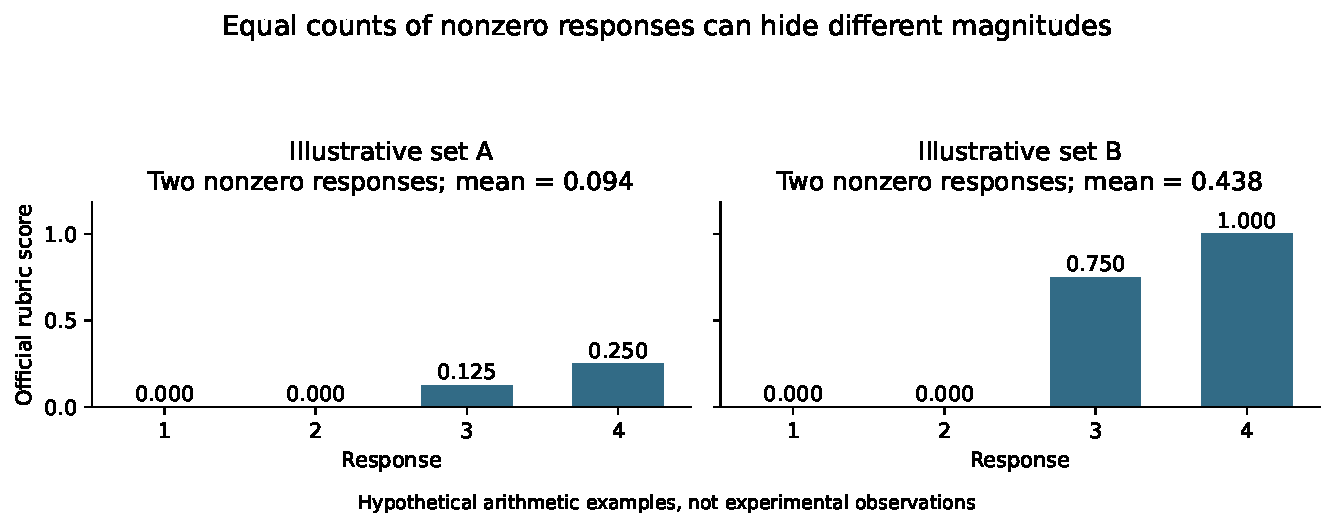
\includegraphics[width=.94\linewidth]{figures/strongreject_magnitude_example.pdf}

\label{fig:strongreject-magnitude-example}\fonte{Prepared by the author (2026).}
\end{figure}

\section{Worked Bootstrap Example}
Alongside the regression, we report mean scores and plots. A mean summarizes the responses we observed, but it can depend on which prompts were evaluated: some requests elicit higher scores than others. We therefore ask how much the mean might change if the evaluation contained a different mix of prompts drawn from the same observed collection. The bootstrap approximates this variation by repeatedly rearranging the sample through random draws. It uses existing scored responses; it does not query the models again.

Figure~\ref{fig:bootstrap-worked-example} traces the calculation from saved responses to the resampled means and interval.

% Generated by eval/scripts/write_bootstrap_example.py.
\paragraph*{A small example with actual scores.} To make the calculation concrete, consider Sagui-7B responses to just three source prompts, 0001, 0002, and 0003, in Portuguese and English. Their observed score pairs (Portuguese, English) are (0.875, 1.000), (0.250, 0.625), and (0.375, 0.250), respectively. Adding all six scores and dividing by six gives the original mean, $3.375/6 = 0.5625$.

If we randomly sample three source-prompt identifiers with replacement, one possible sample is 0001, 0001, and 0003. We include all recorded responses belonging to each selected identifier: the Portuguese and English scores for 0001 appear twice, those for 0003 appear once, and those for 0002 do not appear. This new sample still has six scores, but its mean is $4.375/6 \approx 0.7292$. It is higher because the draw included the higher-scoring prompt 0001 twice and omitted prompt 0002. Another draw could include prompt 0002 twice and give a lower mean. The scores in this example are real; the selected identifiers illustrate the procedure and are not reported analysis replicates.

% Generated by eval/scripts/write_bootstrap_example.py; saved estimates unchanged.
\begin{figure}[p]\centering
\caption[How the prompt-cluster bootstrap works]{From a prompt-group draw to a reported interval. Panel A uses actual scores with an illustrative selection; panel B explains the full procedure. Panel C displays the saved full-model result, not an interval calculated from the three-prompt example.}

\begin{tikzpicture}[x=1cm,y=1cm,font=\fontsize{10}{12}\selectfont,
card/.style={draw=black!20,rounded corners=3pt,text width=3.15cm,minimum height=1.25cm,align=left,inner sep=7pt},
flow/.style={-{Latex[length=2mm]},thick,draw=black!40}]
\definecolor{bootblue}{HTML}{286F8C}
\definecolor{bootorange}{HTML}{A64B39}
\node[anchor=west,font=\bfseries] at (0,0) {A. Example draw};
\node[anchor=west] at (0,-.55) {Saved scores (\texttt{por}, \texttt{eng})};
\node[anchor=west] at (5,-.55) {Selected groups (\texttt{por}, \texttt{eng})};
\node[anchor=west] at (10,-.55) {Recalculate};
\node[card,fill=bootblue!5,anchor=north west] (o0) at (0,-0.9) {\textbf{Prompt 0001}\\(0.875, 1.000)};
\node[card,fill=bootblue!5,anchor=north west] (o1) at (0,-2.5) {\textbf{Prompt 0002}\\(0.250, 0.625)};
\node[card,fill=bootblue!5,anchor=north west] (o2) at (0,-4.1000000000000005) {\textbf{Prompt 0003}\\(0.375, 0.250)};
\node[card,fill=bootorange!8,anchor=north west] (s0) at (5,-0.9) {\textbf{Prompt 0001}\\(0.875, 1.000)};
\node[card,fill=bootorange!8,anchor=north west] (s1) at (5,-2.5) {\textbf{Prompt 0001}\\(0.875, 1.000)};
\node[card,fill=bootblue!5,anchor=north west] (s2) at (5,-4.1000000000000005) {\textbf{Prompt 0003}\\(0.375, 0.250)};
\draw[flow] (o0.east) -- (s0.west);
\draw[flow,draw=bootorange] (o0.east) -- (s1.west);
\draw[flow] (o2.east) -- (s2.west);
\node[anchor=north west,text width=3.8cm,align=left] at (10,-1.05) {\textbf{Original mean}\\[5pt]$3.375/6 = 0.5625$\\[18pt]\textbf{Resampled mean}\\[5pt]$4.375/6 \approx 0.7292$};
\draw[flow] (8.7,-2.9) -- (9.8,-2.9);
\node[anchor=north west,text width=14cm,align=left] at (0,-5.6) {\textbf{What changed?} Prompt 0001 was selected twice; 0002 was omitted. Both language scores travel together.};
\draw[black!25] (0,-6.8) -- (14,-6.8);
\node[anchor=west,font=\bfseries] at (0,-7.3) {B. Repeat on the full scored subset};
\node[anchor=north west,text width=14cm,align=left] at (0,-7.7) {Each draw selects as many groups as the original subset contains, with replacement. Repeat with fresh draws 2\,000 times.};
\node[draw=bootblue!40,fill=bootblue!5,rounded corners=3pt,anchor=north west,text width=13.5cm,align=center,inner sep=8pt] at (0,-9.1) {Draw groups $\longrightarrow$ copy saved responses $\longrightarrow$ one mean\\[5pt]$\mu^{(1)},\ \mu^{(2)},\ \ldots,\ \mu^{(2\,000)}$};
\node[anchor=north west,text width=14cm,align=left] at (0,-10.8) {Order the 2\,000 means. Their 2.5th and 97.5th percentiles give the lower and upper interval endpoints. The reported point estimate is still the original mean.};
\draw[black!25] (0,-12.0) -- (14,-12.0);
\node[anchor=west,font=\bfseries] at (0,-12.5) {C. Reported result: Sagui-7B, 13 languages};
\node[anchor=north west,text width=14cm,align=left] at (0,-12.9) {4\,021 scored responses from 313 source-prompt groups. Saved mean: 0.397; saved 95\% interval: [0.379, 0.415].};
\begin{axis}[at={(.7cm,-14.35cm)},anchor=north west,width=12.6cm,height=1.3cm,scale only axis,
xmin=.35,xmax=.44,ymin=0,ymax=1,axis y line=none,axis x line=bottom,clip=false,
xtick={.35,.38,.41,.44},tick label style={font=\scriptsize},xlabel={Mean StrongREJECT score (detail of the score scale)},label style={font=\scriptsize}]
\addplot[bootblue,very thick,mark=|,mark size=5pt] coordinates {(0.378666,.5) (0.415234,.5)};
\addplot[bootblue,only marks,mark=*,mark size=3pt] coordinates {(0.397072,.5)};
\node[anchor=south,font=\scriptsize] at (axis cs:0.397072,.7) {Original mean};
\end{axis}
\node[anchor=north west,text width=14cm,align=left,font=\fontsize{9}{11}\selectfont] at (0,-16.7) {The interval describes variation under resampling of the observed prompts. It does not correct missing scores or judge errors. No new model answers are generated.};
\end{tikzpicture}

\label{fig:bootstrap-worked-example}\fonte{Prepared by the author (2026).}
\end{figure}


For the reported intervals, we apply this procedure to the full scored subset being summarized. Each draw selects as many prompt identifiers as that subset contains distinct source prompts. Selection is random and allows repetition. Whenever a prompt is selected, we include all its scored responses in that subset, including its different language versions and, where applicable, models. Thus, responses sharing a source prompt remain together. A prompt selected twice contributes its responses twice. We compute one mean from this resample, then start again with a fresh random draw. We repeat these steps 2\,000 times, obtaining 2\,000 resampled means.

To form the reported 95\% interval, we order those means from smallest to largest and use their 2.5th and 97.5th percentiles as the endpoints. Approximately 95\% of the resampled means lie between these endpoints. A narrow interval means that changing the mix of observed prompts changes the mean relatively little; a wide interval means that it changes more. The reported point estimate remains the mean of the original scored responses, not the mean of a particular resample.

This interval captures uncertainty associated with the sampled prompts, conditional on the evaluated models and languages. It does not correct missing scores, validate the judge, or establish that the observed prompts represent every possible harmful request. The fixed random seed, \texttt{20260929}, allows the same random draws to be reproduced. These calculations use frozen responses and form part of the post-review graded-score revision disclosed in Section~\ref{sec:magnitude-method}.

\defensenote{Bootstrap in simple language}{Randomly sample source-prompt identifiers with replacement, keeping all responses to each selected prompt together, then recompute the mean. Repeating this 2\,000 times shows how the mean varies under resampling of the observed prompts. It does not fill missing responses or validate the judge.}


\end{otherlanguage*}
